\documentclass[12pt, a4paper]{article}
\usepackage[utf8]{inputenc}
\usepackage[english]{babel}
\usepackage{fancyhdr}
\usepackage{datetime}
\usepackage{hyperref}
\usepackage{longtable}
\usepackage{graphicx}
\usepackage[font=small,labelfont=bf]{caption}
\hypersetup{
    colorlinks,
    citecolor=black,
    filecolor=black,
    linkcolor=black,
    urlcolor=black
}

\def\labelitemi{--}
\setcounter{tocdepth}{3}
\pagestyle{fancy}
\fancyhf{}
\renewcommand{\headrulewidth}{1pt}
\renewcommand{\footrulewidth}{1pt}
\rhead{\leftmark}
\rfoot{Page \thepage}

\begin{document}

\begin{titlepage}

    \newcommand{\HRule}{\rule{\linewidth}{0.5mm}} % Defines a new command for the horizontal lines, change thickness here
    
    \center % Center everything on the page
     
    %----------------------------------------------------------------------------------------
    %	HEADING SECTIONS
    %----------------------------------------------------------------------------------------
    
    \textsc{\LARGE Università Degli Studi Di Milano}\\[1.5cm] % Name of your university/college
    \textsc{\Large Real-Time Graphics Programming}\\[0.5cm] % Major heading such as course name
    %\textsc{\large Assignment 1}\\[0.5cm] % Minor heading such as course title
    
    %----------------------------------------------------------------------------------------
    %	TITLE SECTION
    %----------------------------------------------------------------------------------------
    
    \HRule \\[0.4cm]
    { \huge \bfseries Real-time autostereogram rendering pipeline }\\[0.4cm] % Title of your document
    \HRule \\[1.5cm]
     
    %----------------------------------------------------------------------------------------
    %	AUTHOR SECTION
    %----------------------------------------------------------------------------------------
    
    \begin{minipage}{0.4\textwidth}
    \begin{flushleft} \large
    \emph{Author:}\\
    Giovanni \textsc{Cocco} \\
    \end{flushleft}
    \end{minipage}
    ~
    \begin{minipage}{0.4\textwidth}
    \begin{flushright} \large
    \emph{Academic year:} \\
    2022-2023\\
    \end{flushright}
    \end{minipage}\\[2cm]
    
    % If you don't want a supervisor, uncomment the two lines below and remove the section above
    %\Large \emph{Author:}\\
    %John \textsc{Smith}\\[3cm] % Your name
    
    %----------------------------------------------------------------------------------------
    %	DATE SECTION
    %----------------------------------------------------------------------------------------
    
    {\large \today}\\[4cm] % Date, change the \today to a set date if you want to be precise
    
    %----------------------------------------------------------------------------------------
    %	LOGO SECTION
    %----------------------------------------------------------------------------------------
    
    
\includegraphics[width=130px, keepaspectratio]{img/unimi.png}\\[1cm] % Include a department/university logo - this will require the graphicx package
     
    %----------------------------------------------------------------------------------------
    
    \vfill % Fill the rest of the page with whitespace
    
    \end{titlepage}

\clearpage
\tableofcontents{}
\listoffigures
\listoftables
\clearpage

\section{Abstract}
In this document we discuss the algorithms, the choices and the implementation details of a real-time autostereogram rendering pipeline built with OpenGL 4.3.\\\\
The pipeline presented allow the rendering of autostereograms starting from a depth buffer that is always produces
as a result on all classical rasterization rendering algorithms. More elaborated effect can be achieved if we supply as input also the color buffer and 
the normal buffer.\\\\
We will first briefly explain what an autostereogram is and how it works from a psychological point of view. We will then discuss a general algorithm to create them.
We will then discuss the implementation detail of the project.\\\\
It should be noted that the input needed for the autostereogram generation algorithm are produced as a result of most real-time rendering pipeline and this 
mean that is possible to apply this technique to an already existent rendering pipeline.\\\\
For this project we made a simple rendering pipeline using Blinn-Phong illumination model, as we will see more sophisticated model give little gain in 
the final result.\\\\
The project also implements blend skinning for skeletal animation, we will discuss the implementation and the difference between linear blend skinning and
dual quaternion skinning.\\\\
We will see how the performance of this pipeline can be totally in the frame budget on most GPU buy may suffer on old laptop one while still
providing 60 frames per second.

\clearpage
\section{Autostereogram}
\subsection{What is an autostereogram}
A stereogram is a 2D image that creates the optical illusion of a 3D scene\footnote{https://en.wikipedia.org/wiki/Autostereogram}. Autostereograms are a particular kind of stereograms
that create this illusion without requiring any additional equipment.\\\\
Our brain is able to perceive depth because each eye receives a different image because they are in slightly different positions on one's head.
We can exploit this behavior by producing one image with repeating patter causing and object to be in the right position from the point of view of each eye
if the eye separation of the subject is the correct one.\\\\
Note that it might take some practice before being able to control the eye separation and be able to see
the optical illusion. For more information on some viewing technique one may take a look at: \url{https://www.hidden-3d.com/how_to_view_stereogram.php}.\\\\
\begin{center}
    \centering
    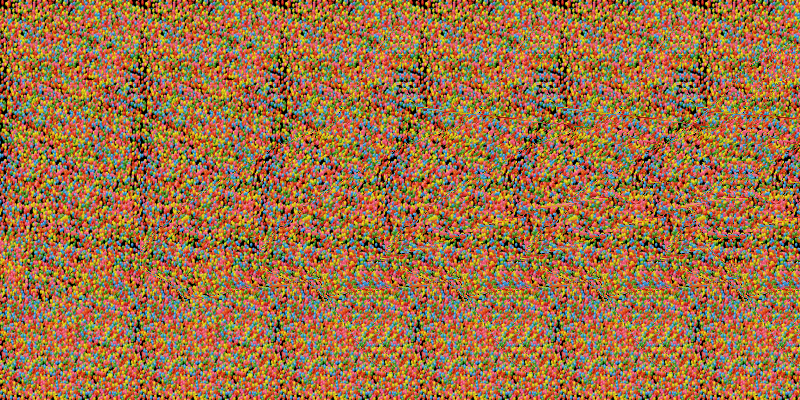
\includegraphics[width=1.0\textwidth]{img/shark.png}
    \captionof{figure}{Autostereogram of a shark}
\end{center}
\clearpage
\subsection{Autostereogram rendering algorithm}
To render an autostereogram we need first to understand the underling geometry.\\
\begin{center}
    \centering
    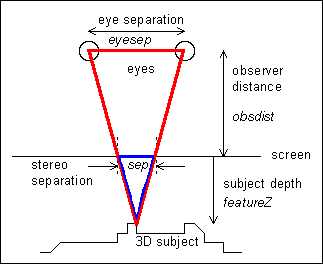
\includegraphics[width=0.7\textwidth]{img/geometry.png}
    \captionof{figure}{The geometry of an autostereogram}
\end{center}
If the two points where the line of sight intercept the screen have the same color the depth of the 3D
subject will be perceived.\\\\
As we can see from the figure the two highlighted triangles have the same angles and as such they are similar.
This means they are proportional, and so we can calculate the separation with the following equation.
\[
sep = \frac{eyesep \cdot featureZ}{featureZ + obsdist}
\]
The general method to create an autostereogram is the following\footnote{http://www.techmind.org/stereo/stech.html}:
\begin{itemize}
    \item Create a depth map of the scene.
    \item For each horizontal line, moving from left to right, and for each point of the depth map link together all the pixel that will have the same color.
    \item Assign to each point a random color making sure the linked one will have the same.
\end{itemize}

\subsection{Advanced effects}
The choice of which color assign to a pixel allow for different effect.\\\\
While it iss possible to use a completely random color is also possible use a texture pattern that will be repeated horizontally.\\\\
It is also possible to highlight the edge of the objects or using a color based on the real object color.
\begin{center}
    \centering
    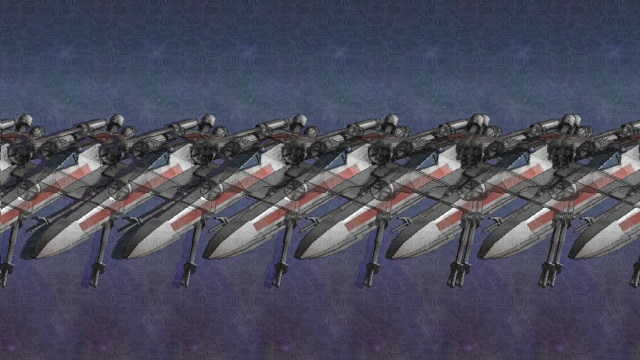
\includegraphics[width=1.0\textwidth]{img/ship.png}
    \captionof{figure}{Object color are used}
\end{center}
As one may expect this means objects will bleed horizontally to other pixels in a repeating fashion.
\section{Scene management}
\subsection{Handle multiple scenes}

\subsection{Assets loading}

\subsection{Object struct}

\subsection{Updating the scene}

\subsection{Camera and input processing}

\section{GUI}

\section{Rendering}
\subsection{Illumination model}

\subsection{Toon shading}

\subsection{Skybox}

\subsection{Autostereogram}

\section{Skeletal animation}

\subsection{Linear blend skinning}

\subsection{Dual quaternion skinning}

\section{Performance evaluation}

\section{Conclusion}

\end{document}